\begin{frame}
    \frametitle{\problemtitle}
    \begin{block}{Problem}
        Find an implicit matching on the set of $n$ bit
        binary strings with $k$ ones, or report that
        no such matching exists.
        Two binary strings are adjacent if one can be 
        transformed into the other by swapping the values
        at two distinct indices.
    \end{block}
    \pause
    \begin{block}{Impossible case}
        A matching does not exist if the number of states
        is odd, i.e. $\binom{n}{k} = 1 \pmod{2}$. In all
        other cases a matching can be created.
    \end{block}
\end{frame}
\begin{frame}
    \frametitle{\problemtitle}
    \begin{block}{Construction}
        There are many solutions. One is to 
        find a Hamiltonian path, then match the 
        $i$-th value to the $(i \oplus 1)$-th.

        \begin{itemize}
            \item Build the Hamiltonian path $H(n, k)$ recursively.
            \item $H(n, k) = 0 H(n-1, k) + 1 H^R(n-1, k-1)$ where $H^R$ is the reversed Hamiltonian path.
        \end{itemize}
        
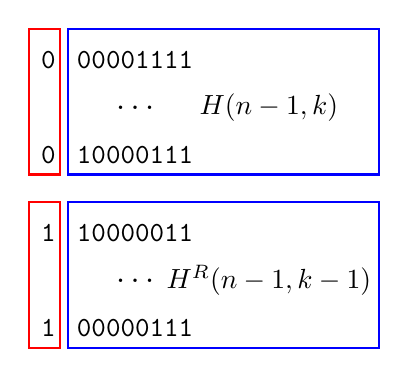
\begin{tikzpicture}[font=\ttfamily]

% --- Top half text ---
\node (t1) at (-0.3,0) {0};
\node (t3) at (-0.3,-1.2) {0};
\node (t12) at (0.8,0) {00001111};
\node (t22) at (0.8,-0.6) {...};
\node (t22) at (2.5,-0.6) {$H(n-1, k)$};
\node (t32) at (0.8,-1.2) {10000111};

% --- Bottom half text ---
\node (b1) at (-0.3,-2.2) {1};
\node (b3) at (-0.3,-3.4) {1};
\node (b12) at (0.8,-2.2) {10000011};
\node (b22) at (0.8,-2.8) {...};
\node (b22) at (2.5,-2.8) {$H^R(n-1, k-1)$};
\node (b32) at (0.8,-3.4) {00000111};

% --- Draw boxes ---
% Top-left box (first column of top half)
\draw[red, thick] (-0.55,0.4) rectangle (-0.15,-1.45);

% Top-right box (rest of top half)
\draw[blue, thick] (-0.05,0.4) rectangle (3.9,-1.45);

% Bottom-left box (first column of bottom half)
\draw[red, thick] (-0.55,-1.8) rectangle (-0.15,-3.65);

% Bottom-right box (rest of bottom half)
\draw[blue, thick] (-0.05,-1.8) rectangle (3.9,-3.65);

\end{tikzpicture}

    \end{block}
\end{frame}



\begin{frame}
    \frametitle{\problemtitle}
    \begin{block}{Runtime}
        Runtime $\mathcal{O}(n)$ if done well, $\mathcal{O}(n^2)$ also passes.
    \end{block}
    \pause
    \solvestats
\end{frame}
